\documentclass[a4paper,twoside]{article}
\usepackage{autiwa}

\title{Aide mémoire Git}
\author{Autiwa}

\newcommand{\raccourci}[1]{{\bfseries #1}}

\makeindex
\begin{document}

\tableofcontents

\clearpage

\section{Préambule}
Git permet de gérer un projet (de programmation généralement) et de garder en mémoire l'historique de toutes les versions d'un ensemble de fichiers. Il permet de gérer un projet à plusieurs, de programmer afin de pouvoir revenir en arrière, comparer avec d'anciennes versions et cie. 

Le principe est d'avoir un serveur git (un seul possible) qui va garder en mémoire l'historique de toutes les versions et un client git (plusieurs possibles) qui vont se connecter au serveur pour mettre à jour la version des fichiers ou en récupérer les dernières versions.

\begin{remarque}
Il est possible que le serveur soit lui aussi client, dans le cas où il n'y aurait qu'un seul développeur et qu'on ne souhaite pas passer par internet.
\end{remarque}

\subsection{Configuration}
Afin d'avoir la coloration syntaxique, il faut faire : 
\begin{verbatim}
git config --global color.diff auto
git config --global color.status auto
git config --global color.branch auto
\end{verbatim}

De même, il faut configurer votre nom (ou pseudo) :
\begin{verbatim}
git config --global user.name "votre_pseudo"
\end{verbatim}


Puis votre e-mail :
\begin{verbatim}
git config --global user.email moi@email.com
\end{verbatim}


Vous pouvez aussi éditer votre fichier de configuration .gitconfig situé dans votre répertoire personnel pour y ajouter une section alias à la fin :
\begin{verbatim}
vim ~/.gitconfig
\end{verbatim}

\begin{verbatim}
[color]
        diff = auto
        status = auto
        branch = auto
[user]
        name = votre_pseudo
        email = moi@email.com
[alias]
        ci = commit
        co = checkout
        st = status
        br = branch
\end{verbatim}

\subsection{Git sur internet}
Je vais prendre l'exemple de google code, qui est celui que j'ai choisi et que je suis en train d'apprendre.


Une fois le projet créé (sur la page \url{http://code.google.com/hosting/createProject}), il faut faire la commande suivante pour récupérer le contenu du projet localement (et pouvoir envoyer les modifs par la suite) : 
\begin{verbatim}
cd Formulaire
git clone https://autiwa@code.google.com/p/autiwa-tutorials/ 
\end{verbatim}\index{git!clone}

Cette commande permet de récupérer le contenu du projet et de le copier dans un dossier \textbf{Formulaires} qui sera créé dans le dossier courant.

\begin{definition}[Clone]
Opération d'extraction d'une version d'un projet du repository vers un répertoire de travail local.
\end{definition}


\subsection{Git localement}\label{sec:git_init}
Le serveur ET le client seront alors sur la même machine. Pour créer un projet, il faut créer un dossier, par exemple dans mon cas un dossier \textbf{mercury} dans mon \textbf{\$HOME}, puis je fais, dans mon répertoire utilisateur : 
\begin{verbatim}
cd mercury
git init
\end{verbatim}
pour un projet que j'appelle \textbf{mercury}.

\section{Commandes universelles git}
Ici, je note les commandes qui sont valables à la fois pour svn installé sur un serveur internet, ou sur une machine locale pour un usage personnel.

\subsection{Commandes de base}

\subsubsection{Ajouter des fichiers ou dossiers au projet : add}\index{git!add} \index{Ajouter des fichiers}
Pour ajouter des fichiers il faut faire :
\begin{verbatim}
git add latex/ vim/ 
\end{verbatim}
où \textbf{latex/} et \textbf{vim/} sont deux dossiers existant dans le dossier local de référence

\begin{remarque}
Au cas où ça serait pas clair. J'ai créé un dossier \textbf{/home/autiwa/Formulaires} grâce à \refsec{sec:git_init}. Dans ce dossier, j'ai créé et rempli à la main les sous-dossiers \textbf{latex/} et \textbf{vim/}. Maintenant, grâce à la commande ci-dessus, je définis ces sous-dossiers comme étant rattachés au projet. En faisant ainsi le contenu est rajouté récursivement.
\end{remarque}

\begin{attention}
Cette commande n'agit que sur le répertoire local (la \emph{working copy}). Il faut ensuite appliquer ces changements au dépot (voir \refsec{sec:commit}) pour les valider.
\end{attention}

\bigskip

Supposons que vous veniez d'ajouter un fichier à Git avec git add et que vous vous apprêtiez à le \og commiter \fg. Cependant, vous vous rendez compte que ce fichier est une mauvaise idée et vous voudriez annuler votre git add.

Il est possible de retirer un fichier qui avait été ajouté pour être \og commité \fg en procédant comme suit :
\begin{verbatim}
git reset HEAD -- fichier_a_supprimer
\end{verbatim}

\subsubsection{Enregistrer les modifications localement : commit}\index{git!commit}\index{mise à jour local -> serveur}\label{sec:commit}

Pour mettre à jour les versions sur serveur à partir des modifications effectuées localement, il faut sélectionner les fichiers qu'on veut ajouter au prochain commit avec \textbf{git add} puis faire le commit :
\begin{verbatim}
git add FILE
git commit -m "initialisation"
\end{verbatim}
où \textbf{"initialisation"} est le commentaire qui décrit la mise à jour et les modifications effectuées. \textbf{FILE} peut être un ou plusieurs fichiers, l'astérisque pouvant être utilisée.

À noter que l'option -a permet de se passer du \textbf{git add} et d'ajouter automatiquement tous les fichiers qui ont été modifiés :
 \begin{verbatim}
git commit -a -m "initialisation"
\end{verbatim}

\begin{remarque}
Si on a fait un 'add' par erreur et qu'on ne veut pas ajouter un certain fichier au prochain commit, il suffit de faire :
\begin{verbatim}
git reset FILE
\end{verbatim}
\end{remarque}

\bigskip

\begin{attention}
Un commit avec git est local : à moins d'envoyer ce commit sur le serveur comme on apprendra à le faire plus loin, personne ne sait que vous avez fait ce commit pour le moment. Cela a un avantage : si vous vous rendez compte que vous avez fait une erreur dans votre dernier commit, vous avez la possibilité de l'annuler (ce qui n'est pas le cas avec SVN !).
\end{attention}

\subsubsection{Identifier un commit}
Pour indiquer à quel commit on souhaite revenir, il existe plusieurs notations :
\begin{itemize}
\item \verb|HEAD| : dernier commit ;
\item \verb|HEAD^| : avant-dernier commit ;
\item \verb|HEAD^^| : avant-avant-dernier commit ;
\item \verb|HEAD~2| : avant-avant-dernier commit (notation équivalente) ;
\item \verb|d6d98923868578a7f38dea79833b56d0326fcba1| : indique un numéro de commit précis ;
\item \verb|d6d9892| : indique un numéro de commit précis (notation équivalente à la précédente, bien souvent écrire les premiers chiffres est suffisant tant qu'aucun autre commit ne commence par les mêmes chiffres).
\end{itemize}

\begin{exemple}
\begin{verbatim}
git diff HEAD^
\end{verbatim}
permet de comparer la version courante avec la version juste avant.
\end{exemple}

\subsubsection{Mettre à jour sa copie locale : pull}\index{git!pull} \index{Mise à jour du dépôt}
\begin{verbatim}
git pull
\end{verbatim}

Pour celà, il faut que le dossier dans lequel on se trouve ait déjà été défini comme un dossier git via un \gras[commande git!clone]{clone} (voir \refsec{sec:git_init})

\subsubsection{Propager les modifications locales sur le dépot du serveur : push}\index{git!push}
On peut modifier ces commits là, tant qu'ils sont en local. Puis une fois vérifié. Il ne reste plus qu'à les envoyer sur le serveur. Pour celà on vérifie tout d'abord ce qu'on s'apprête à envoyer, et on envoie sur le serveur : 
\begin{verbatim}
git log -p
git push
\end{verbatim}

\subsection{Annuler ou nettoyer}
\subsubsection{Annuler les modifications non commités : checkout}
Pour annuler les modifications locales et revenir à la dernière révision : 
\begin{verbatim}
git checkout *.f90
\end{verbatim}\index{git!checkout}
va remettre en l'état tous les fichiers du dépot qui sont présents dans le dossier courant (on peut aussi ne préciser qu'un seul fichier).

\subsubsection{Annuler un git add : git reset}\index{git!add}
Parfois, on peut avoir préparé des modifications à ajouter à un commit, via \textbf{git add}, soit sur des fichiers déjà suivis, soit pour suivre de nouveaux fichiers. Afin de retirer certains de ces fichiers de la liste des fichiers pour le prochain commit, il faut faire :
\begin{verbatim}
git reset HEAD <FILE>
\end{verbatim}\index{git!reset}

\subsubsection{Annuler un commit effectué par erreur}
\subsubsection{Modifier le message du dernier commit}
Valable si on n'a pas fait de \gras[git!push]{git push} :
\begin{verbatim}
git commit --amend
\end{verbatim}

\subsubsection{Annuler un commit pas encore publié}\index{git!reset}
Valable si on n'a pas fait de \gras[git!push]{git push} :
\begin{verbatim}
git reset HEAD^
\end{verbatim}
annule le dernier commit et revient à l'avant dernier. Pour autant les fichiers ne sont pas modifiés, seul le commit en lui même est annulé.

\bigskip

Pour annuler les modifications liées au commit, il faut faire un hard reset :
\begin{verbatim}
git reset --hard HEAD^
\end{verbatim}\index{git!reset}
Annule le dernier commit et toutes les modifications qui s'y rapportent. 

\subsubsection{Annuler un commit publié}
Si vous publiez un commit sur le serveur, mais que vous souhaitez l'annuler, c'est quand même possible, mais c'est un peu plus barbare qu'un commit non encore propagé (à l'aide de push). 

Pour celà il faut créer un nouveau commit qui annule les modifications du commit que vous souhaitez annuler. Il faut alors connaître l'ID du commit visé et faire : 
\begin{verbatim}
git revert 6261cc2
\end{verbatim}
Il faut préciser l'ID du commit à \og revert \fg. Il n'est pas obligatoire d'indiquer l'ID en entier (qui est un peu long), il suffit de mettre les premiers chiffres tant qu'ils sont uniques (les 4-5 premiers chiffres devraient suffire). On vous invite à entrer un message de commit. Un message par défaut est indiqué dans l'éditeur.

Une fois que c'est enregistré, le commit d'annulation est créé. Il ne vous reste plus qu'à vérifier que tout est bon et à le publier (avec un git push).

\subsubsection{Mettre de coté et reprendre un travail en cours : stash}\index{git!stash}
Si on est en train de faire une modification, sans faire de commit, mais qu'on doit faire des modifications plus urgentes, et surtout immédiate, on peut souhaiter ne pas perdre le travail déjà effectué. Au lieu de faire un commit on peut simplement faire une sauvegarde de l'état modifié, pour le restituer plus tard.

\begin{verbatim}
git stash save "ongoing work about something"
\end{verbatim}
va sauvegarder les modifications effectuées depuis le dernier commit dans le \textbf{stash}, et remettre les fichiers dans leur état lors du dernier commit. 

On peut ensuite faire les modifications urgente, dans cette branche ou dans une autre, faire des commit etc. Puis une fois qu'on veut réutiliser le stash, il suffit de faire : 
\begin{verbatim}
git stash apply
\end{verbatim}

\subsubsection{Supprimer les fichiers inconnus de Git}\index{git!clean}
Pour supprimer les fichiers \textbf{untracked}, il faut utiliser la commande \gras[git!clean]{clean}. 

D'abord on simule la suppression pour voir ce qu'il va supprimer (option \textbf{-n}) :
\begin{verbatim}
git clean -n
\end{verbatim}

\begin{itemize}
\item[\textbf{-d}] Pour supprimer aussi les dossiers
\item[\textbf{-x}] Pour supprimer les fichiers ignorés par Git (\textbf{.gitignore})
\item[\textbf{-X}] Pour \textbf{ne} supprimer \textbf{que} les fichiers ignorés par Git (\textbf{.gitignore})
\item[\textbf{-f}] Par défaut, il faut cette option pour supprimer les fichiers, ça évite de faire le nettoyage par erreur.
\end{itemize}

Pour supprimer les fichiers, une fois qu'on a vu ce qu'il allait faire :
\begin{verbatim}
git clean -f
\end{verbatim}
ou
\begin{verbatim}
git clean -f <PATH>
\end{verbatim}
si on souhaite faire cela dans un dossier particulier.


\subsection{Contrôler}
\subsubsection{État du dépot local (modifications par rapport au dernier commit) : status}\index{git!status}
La commande git status vous indique les fichiers que vous avez modifiés récemment :
\begin{verbatim}
$ git status
# On branch master
nothing to commit (working directory clean)
\end{verbatim}

\subsubsection{Historique des modifications : log}\index{historique des modifications}\index{git!log}
La commande \texttt{log} permet de voir un historique des commentaires de révision, soit de l'ensemble des fichiers, soit d'un fichier en particulier.

\begin{verbatim}
git log
\end{verbatim}\index{git!log}
affiche l'historique de toutes les révisions.

\begin{attention}
Chaque commit est numéroté grâce à un long numéro hexadécimal comme 12328a1bcbf231da\-8eaf942f8d68c7dc0c7c4f38. Cela permet de les identifier.
\end{attention}

Pour avoir les informations d'un commit particulier, il faut faire :
\begin{verbatim}
git show 99adb32062d66121f2ba056dc820b9529a9ea08c
\end{verbatim}\index{git!show}

\subsubsection{Différences entre versions : diff}

\begin{verbatim}
git diff
\end{verbatim}

\begin{remarque}
Il est possible de regarder les différences sur un fichier en particulier.
\end{remarque}

Pour regarder les différences avec le commit précédent, il suffit de faire :
\begin{verbatim}
git diff HEAD^
\end{verbatim}

\bigskip

On peut faire des diff entre des branches 
\begin{verbatim}
git diff master branch_devel
\end{verbatim}
ou entre deux versions en spécifiant leur hashtag : 
\begin{verbatim}
git diff dqsfg54qsdf35dqs4f ze9r8az7er3azer2
\end{verbatim}

J'utilise personnellement \gras[git!difftool]{difftool}, ça me permet d'utiliser \gras{meld} que j'affectionne particulièrement.

\subsubsection{Revenir à une révision antérieure : checkout}\label{sec:revenir_en_arriere}\index{git!checkout}
Pour changer la révision courante, il suffit de faire : 
\begin{verbatim}
git checkout c23db4a1d05e
\end{verbatim}
et la révision \textbf{c23db4a1d05e} devient la révision active. 

Pour revenir à la dernière révision d'une branche donnée, il suffit de faire :
\begin{verbatim}
git checkout nom_de_branche
\end{verbatim}
ainsi
\begin{verbatim}
git checkout master
\end{verbatim}
active la dernière révision de la branche principale.



\section{Travailler avec des branches : branch}\index{git!branch}
\begin{figure}[htb]
\centering
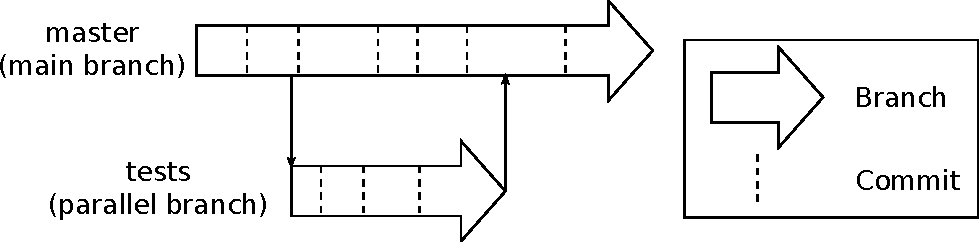
\includegraphics[width=0.75\linewidth]{figure/branchs.pdf}
\caption{Le principe des branches est de travailler à part sur des modifications et de ne les fusionner avec la branche principale que si c'est ok et ça donne quelque chose.}
\end{figure}

L'idée derrière le fait de créer des branches, c'est de bien séparer les idées de développement, et de pouvoir les tester et les séparer avant de les inclure (ou pas) dans la branche principale. 

\begin{important}
En gros, Si vous avez une modification à faire, qui risque de prendre un peu de temps et qui va nécessiter plusieurs commit, faites une branche !
\end{important}


\subsection{Lister les branches}
Première chose utile, lister les branches existantes. Par défaut il n'y aura que la branche principale : 
\begin{verbatim}
git branch
\end{verbatim}

\subsection{Créer une branche}
Pour créer une branche \textbf{test\_01}, il faut utiliser la commande :
\begin{verbatim}
git branch test_01
\end{verbatim}

Si vous listez alors les branches, vous aurez :
\begin{verbatim}
$ git branch
* master
  test_01
\end{verbatim}
où on voit que \textbf{master} est toujours la branche active. Il faut donc changer de branche pour pouvoir modifier les fichiers et faire des commits dans cette branche.

\subsection{Gérer une branche distante}
Pour que cette branche soit envoyée et synchronisée avec le dépot distant, si on veut en fair eune branche permanente, il faut lancer la commande :
\begin{verbatim}
git push origin test_01
\end{verbatim}\index{branche distance}

Pour que quelqu'un puisse \textbf{suivre} les modifications de cette branche, il devra utiliser la commande suivante :
\begin{verbatim}
git checkout -b ma-branche origin/ma-branche
\end{verbatim}

Ce qui revient à créer dans le nouveau dépôt créé une branche \textbf{ma-branche} qui suivra celle du dépôt distant \textbf{origin/ma-branche}.

\bigskip

On peut de plus supprimer une branche distante en faisant : 
\begin{verbatim}
git push origin :test_01
\end{verbatim}\index{branche distance}

\subsection{Aller dans une branche et y faire des commits}
Il faut déclarer cette branche comme active via :
\begin{verbatim}
git checkout test_01
\end{verbatim}

La liste des branches donne alors :
\begin{verbatim}
$ git branch
  master
* test_01
\end{verbatim}
qui montre que la branche \textbf{test\_01} est maintenant active.

\begin{remarque}
\textbf{git checkout} est utilisé pour changer de branche mais aussi pour restaurer un fichier tel qu'il était lors du dernier commit. La commande a donc un double usage.
\end{remarque}

\begin{attention}
Vous pouvez changer d'une branche à l'autre, faire des commits (éventuellement des push) sur la branche principale, mais ceux ci ne seront pas propagés aux autres branches, c'est d'ailleurs le principe des branches. 
\end{attention}

\subsection{Fusionner une branche avec la branche principale}
Pour celà, il faut se placer dans la branche principale et demander d'intégrer les changements d'une autre branche en faisant : 
\begin{verbatim}
git checkout master
git merge test_01
\end{verbatim}

Une fois fusionné, vous pouvez supprimer la branche \textbf{test\_01} (voir la section suivante).

\subsection{Incorporer les nouvelles modifications de la branche principale dans une branche annexe : rebase}\index{git!rebase}
\begin{figure}[htb]
\centering
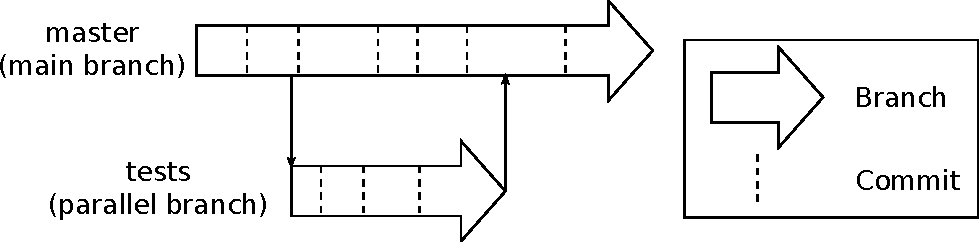
\includegraphics[width=0.75\linewidth]{figure/branchs.pdf}
\caption{Avec git rebase, on peut inclure les dernières modifications d'une branche dans une autre branche, afin de décaler la \og base\fg de cette branche. En résumé, c'est comme si on faisait bifurquer la branche concernée à la fin de la branche de laquelle on veut inclure les modifications}
\end{figure}



Pour inclure les dernières modifications de \textbf{master} dans \textbf{devel}, il faut se placer dans la branche \textbf{devel}, et faire :
\begin{verbatim}
git rebase master
\end{verbatim}


\begin{verbatim}
git rebase master devel
\end{verbatim}
permet d'inclure dans \textbf{devel} les dernières modifications de \textbf{master} quelle que soit la branche courante.
\bigskip

En cas de conflits, on peut modifier les fichiers affectés et continuer via la commande 
\begin{verbatim}
git rebase --continue
\end{verbatim}
ou annuler directement avec la commande
\begin{verbatim}
git rebase --abort
\end{verbatim}

\subsection{Supprimer une branche}
Pour supprimer une branche dont vous avez déjà propagé les modifications dans la branche principale, faites : 
\begin{verbatim}
git branch -d test_01
\end{verbatim}

Si jamais vous souhaitez supprimer une branche sans avoir propagé les changements (si cet essai était une erreur par exemple) vous pouvez utiliser la commande suivante qui force la suppression : 
\begin{verbatim}
git branch -D test_01
\end{verbatim}

\section{Gérer un conflit}
Un conflit survient quand on veut mettre à jour le dépot : 
\begin{verbatim}
git pull
remote: Counting objects: 7, done.
remote: Finding sources: 100% (7/7), done.
remote: Total 7 (delta 0)
Unpacking objects: 100% (7/7), done.
From https://code.google.com/p/blablabla
   93ad6a9..a10e8d1  master     -> origin/master
Auto-merging recettes/recettes.pdf
CONFLICT (content): Merge conflict in recettes/recettes.pdf
Automatic merge failed; fix conflicts and then commit the result.
\end{verbatim}

L'idée pour résoudre le conflit est de modifier le fichier de conflit, soit en choisissant \textbf{--ours} ou \textbf{--theirs}, soit en utilisant \textbf{mergetool}, puis d'ajouter le fichier au dépot via un nouveau commit, et ensuite d'essayer de mettre à jour de nouveau.

\subsection{Écraser un fichier par un autre}
On peut garder soit le fichier local, soit le fichier distant. C'est la partie la plus facile. Pour garder notre fichier :
\begin{verbatim}
git checkout --ours filename.c
git add filename.c
git commit -m "using theirs"
\end{verbatim}

Pour garder leur version :
\begin{verbatim}
git checkout --theirs filename.c
git add filename.c
git commit -m "using theirs"
\end{verbatim}

\subsection{Regarder les différences et en tenir compte}
Si on veut voir le contenu des fichiers et créer notre futur fichier à partir des deux fichiers du conflit, on a :
\begin{verbatim}
git mergetool
\end{verbatim}

Mais ceci ne va fonctionner qu'avec des fichier ASCII. Dans mon cas, j'avais un conflit avec un fichier .pdf, et dans ce cas, mergetool ne fonctionne pas, il faut choisir si on veut le fichier distant ou le fichier local. Dans tous les cas ce sont normalement des fichiers qui sont aisément générable, le soucis majeur étant de ne plus être embêté par le conflit.

\begin{remarque}
J'utilise \textbf{meld}, que j'aime beaucoup, et qui marche autant pour les diff (\textbf{difftool}) que pour les conflits (\textbf{mergetool}).
\end{remarque}

\section{Avancé}
\subsection{Tagger une version : tag}\index{git!tag}
Il est possible d'associer un tag (un nom de code) à un commit particulier, afin de le mettre en valeur, pour lui donner un numéro de version par exemple, pour les versions stables que les gens devraient utiliser.

Pour ajouter un tag sur un commit :
\begin{verbatim}
git tag NOMTAG IDCOMMIT
\end{verbatim}
ou avec un message explicatif :
\begin{verbatim}
git tag NOMTAG IDCOMMIT -m "message associe au tag"
\end{verbatim}


Donc dans le cas présent, on écrirait :
\begin{verbatim}
git tag v1.3 2f7c8b3428aca535fdc970feeb4c09efa33d809e
\end{verbatim}

Un tag n'est pas envoyé lors d'un push, il faut préciser l'option \textbf{--tags} pour que ce soit le cas :
\begin{verbatim}
git push --tags
\end{verbatim}

Maintenant, tout le monde peut référencer ce commit par ce nom plutôt que par son numéro de révision.

\bigskip

Pour supprimer un tag créé :
\begin{verbatim}
git tag -d NOMTAG
\end{verbatim}

\bigskip

Pour lister les tags existants :
\begin{verbatim}
git tag -l
\end{verbatim}

On peut aussi lister les tags correspondant à un motif particulier : 
\begin{verbatim}
$ git tag -l 'v1.4.2.*'
v1.4.2.1
v1.4.2.2
v1.4.2.3
v1.4.2.4
\end{verbatim}

\bigskip

Pour avoir les infos sur le tag \textbf{nomdutag} : 
\begin{verbatim}
git show nomdutag
\end{verbatim}



\subsection{Ignorer des fichiers (.gitignore)}\index{.gitignore}\label{sec:gitignore}
Pour ignorer un fichier dans git, créez un fichier \textbf{.gitignore} (à la racine) et indiquez-y le nom du fichier. Entrez un nom de fichier par ligne, comme ceci :
\begin{verbatim}
project.xml
dossier/temp.txt
*.tmp
cache/*
\end{verbatim}
Aucun de ces fichiers n'apparaîtra dans git status, même s'il est modifié. Il ne paraîtra donc pas dans les commits.
Utilisez cela sur les fichiers temporaires par exemple, qui n'ont aucune raison d'apparaître dans Git.

Il est possible d'utiliser une étoile (*) comme joker. Dans l'exemple précédent, tous les fichiers ayant l'extension \textbf{.tmp} seront ignorés, de même que tous les fichiers du dossier cache.

\subsection{Rechercher dans les fichiers du dépot : git grep}\index{git!grep}
On peut vouloir chercher quelque chose parmis les fichiers du dépot. Une commande très simple pour faire ça : 
\begin{verbatim}
git grep "xmax"
\end{verbatim}
qui va donner toutes les occurences par fichier. Mais si on veut aussi les numéros de lignes, il suffit alors de faire :
\begin{verbatim}
git grep -n "xmax"
\end{verbatim}

\begin{remarque}
À noter que les expressions régulières sont possibles.
\end{remarque}

\subsection{Rechercher un bug en utilisant la puissance de GIT : bisect}\index{git!bisect}
J'ai eu le cas tout à l'heure et j'ai découvert la puissance de \textbf{bisect}, je vais tâcher de l'expliquer du mieux possible. Vous avez un bug dans votre code, vous ne savez pas d'où vient le bug, \textbf{bisect} est fait pour vous. 

Le principe est le suivant : Vous avez une révision que vous savez ne pas fonctionner (la dernière par exemple) et une qui fonctionne (au pire la première si vous en avez peu, sinon vous en trouvez une assez ancienne et qui fonctionne. Personnellement j'ai fini par y aller franco, et je suis remonté six mois en arrière, une centaine de révisions à tester, mais avec \textbf{bisect} c'est rapide. Pour trouver cette révision, j'ai fait \textbf{git checkout} (qui permet de revenir à une révision antérieure \refsec{sec:revenir_en_arriere}) jusqu'à ce que je trouve une révision qui fonctionne. 

Une fois fait, on peut exploiter la puissance de \textbf{bisect}, qui va nous aider à trouver par dichotomie la révision qui a introduit le bug. On part donc d'un encadrement en ayant une version bonne de référence et une version mauvaise, et on sait donc que la révision fautive se trouve au milieu.

\bigskip

La première étape est d'avoir une version de référence propre, il ne faut pas qu'il reste des modifications non encore sauvées dans un commit. Si vous voulez mettre des modifs de cotés, utilisez \textbf{git stash} : 
\begin{verbatim}
git stash
\end{verbatim}\index{git!stash}

Ensuite, on démarre l'opération de traque du bug via :
\begin{verbatim}
git bisect start
\end{verbatim}

On déclare le \textbf{mauvais} commit :
\begin{verbatim}
git bisect bad # le commit actuel
\end{verbatim}

On déclare le \textbf{bon} commit : 
\begin{verbatim}
git bisect good 3776c939294f
\end{verbatim}
où \textbf{3776c939294f} est la référence du commit en question. 

\bigskip

Une fois fait, vous aurez un message qui ressemblera à ça :
\begin{verbatim}
Bisecting: 65 revisions left to test after this
\end{verbatim}

\textbf{bisect} nous place automatiquement dans des commit différents, indique combien il reste de révisions à tester, et le nombre d'étape estimée pour arriver à trouver l'origine du bug. 

Vous devez donc tester si cette version bugue ou pas. L'idéal est d'avoir un script qui permet de voir rapidement si ça bugue. J'avais pour ma part un script python de tests unitaires que je lançais à chaque fois. 

Une fois que vous savez si la version courante bugue ou pas, il suffit de le dire à bisect via : 
\begin{verbatim}
git bisect good
\end{verbatim}
ou
\begin{verbatim}
git bisect bad
\end{verbatim}
et en fonction de ça, bisect vous mettre une autre révision à tester. Une fois qu'il aura trouvé LA révision fautive, il le dira par :
\begin{verbatim}
d109d47732cb85652b79d679edd7bfe2379e5707 is first bad commit
\end{verbatim}

\begin{attention}
Si pour une raison ou pour une autre, un commit particulier vous pose problème (problème de compilation ou impossibilité de tester, il est possible de dire à bisect qu'on souhaite passer ce commit et en tester un autre à la place via :
\begin{verbatim}
git bisect skip
\end{verbatim}
\end{attention}


\begin{important}
Pendant la bisection, git créé une branche spéciale dédiée. N’oubliez pas de repasser sur votre branche de développement quand vous aurez débusqué la régression. Il est possible de le faire simplement en tapant :
\begin{verbatim}
git bisect reset
\end{verbatim}
\end{important}

\begin{remarque}
La première fois où j'ai utilisé bisect, j'ai oublié de faire \textbf{git bisect reset} et je me suis retrouvé sur une branche \textbf{(no branch)} sans m'en rendre compte. J'ai donc fait des modifications là, sans réaliser que je ne modifiais plus \textbf{master}. Pour plus d'infos quant à la solution à ce problème, voir \refsec{sec:no-branch}.
\end{remarque}

\bigskip

Pour aller plus loin, il est possible de carrément automatiser la tâche si vous arrivez à faire un script qui peut tester le bug, et qui retourne 0 si le code est correct, 1 si le code est incorrect, et 125 si on ne peut pas tester le code (\textbf{git skip}). Pour le faire, il suffit de procéder ainsi :
\begin{verbatim}
git bisect start HEAD <bad_commit> -- # raccourci
git bisect run script
\end{verbatim}

\subsection{Afficher la branche dans le prompt de la console}
Avec Bash, il est possible d'afficher la branche active quand on arrive dans une partie sous gestionnaire de version GIT avec la commande suivante, rajoutée dans le \textbf{.bash\_profile} ou le \textbf{.bashrc} : 
\begin{lstlisting}[language=bash]
git_branch_name_prompt() {
    git_status_output=$(git status 2> /dev/null) || return

    branch_name() {
        sed -n 's/# On branch //p' <<< "$git_status_output"
    }

    echo -e "($(branch_name))"
}

git_branch_colour_prompt() {
    git_status_output=$(git status 2> /dev/null) || return

    find_pattern_in_status() {
        local pattern="$1"
        [[ "$git_status_output" =~ ${pattern} ]]
    }

    is_clean() {
        find_pattern_in_status '(working directory clean)'
    }

    is_local_changes() {
        local added='# Changes to be committed'
        local not_added='# Changes not staged for commit'
        find_pattern_in_status "($added|$not_added)"
    }

    is_untracked() {
        find_pattern_in_status '# Untracked files'
    }

    # local bold="\033[1m"
    local no_colour="\033[0m"

    local red="\033[31m"
    local green="\033[32m"
    local yellow="\033[33m"
    local branch_colour=""

    if is_untracked
    then
        branch_colour=$red
    elif is_local_changes
    then
        branch_colour=$yellow
    elif is_clean
    then
        branch_colour=$green
    fi
    # echo -e "$branch_colour$(branch_name)$no_colour"
    echo -e "$branch_colour"
}

PS1="\h.\u\[\$(git_branch_colour_prompt)\]\$(git_branch_name_prompt)\[\033[0m\]> "
\end{lstlisting}

Le résultat sera alors :
\begin{verbatim}
arguin.login(master)> 
\end{verbatim}
si on est dans un dossier GIT, \textbf{master} étant le nom de la branche active, et :
\begin{verbatim}
arguin.login> 
\end{verbatim}
si le dossier courant n'est pas un dossier GIT.

La couleur sera fonction du status du dépot. Si le dépot est à jour, ce sera vert, s'il y a eu des changements locaux, jaune, et s'il y a eu des commits locaux qui n'ont pas encore été propagés (push), ce sera orange. S'il y a des fichiers qui ne sont pas suivis, ce sera rouge (pour ignorer des fichiers il faut se servir du fichier .gitignore, voir \refsec{sec:gitignore}).

\begin{remarque}
La difficulté est ici d'afficher les couleurs. Il faut échapper ces caractères pour que le retour à la ligne et l'effacement de la ligne se fasse de manière correcte. On est ainsi obligé d'afficher et d'échapper les couleurs au tout dernier moment, dans PS1, et on ne peut donc pas encapsuler ces fonctions dans une grosse fonction qu'on appelerait par la suite.
\end{remarque}

\subsection{branche (no branch), récupérer les commits}\label{sec:no-branch}
Par exemple avec bisect, on peut sans faire exprès faire des commits dans une branche \textbf{(no branch)} et se retrouver dans \textbf{master} sans rien de nouveau. Passé le coup de stress, voici ce qu'on peut faire pour facilement récupérer les données. 

La commande \textbf{reflog} permet d'avoir un historique de ce qu'on a fait et donc de récupérer le \textbf{hash-ID} de la branche \textbf{(no branch)} qui n'apparait plus une fois qu'on est repassé dans \textbf{master} : 
\begin{footnotesize}
\begin{verbatim}
$ git reflog
934101e HEAD@{0}: commit: improving some scripts
c23db4a HEAD@{1}: checkout: moving from 99adb32062d66121f2ba056dc820b9529a9ea08c to master
99adb32 HEAD@{2}: commit: improving some scripts
70ca613 HEAD@{3}: commit: Modification of the formula for the feedback of the eccentricity
\end{verbatim}
\end{footnotesize}

La ligne qui nous intéresse est celle-ci :
\begin{verbatim}
checkout: moving from 99adb32062d66121f2ba056dc820b9529a9ea08c to master
\end{verbatim}
C'est la ligne qui montre où on est passé depuis \textbf{(no branch)} jusqu'à \textbf{master}, en faisant 
\begin{verbatim}
git checkout master
\end{verbatim}
\begin{remarque}
Si on est encore dans \textbf{(no branch)} on peut directement noter de \textbf{hash-ID} en fait.
\end{remarque}

Une fois dans master, on peut alors faire : 
\begin{verbatim}
git merge 99adb32062d66121f2ba056dc820b9529a9ea08c
\end{verbatim}
pour récupérer toutes les modifications de cette branche.

\subsection{Créer des patchs et les appliquer}
Il est possible de créer des patchs, qui vont contenir différentes modifications à appliquer où on veut. Dans la pratique, je me suis servi de ça pour appliquer des modifications sur certains fichiers (sur plusieurs centaines de révisions) afin de déporter ces modifications sur une autre branche. 

Pour faire court, si on veut suivre les modifications d'un ou plusieurs fichiers bien précis (et ignorer les autres) pour appliquer ces modifications ailleurs, il faut faire : 
\begin{verbatim}
git format-patch --output-directory myPatch 7552b3a2fb57..dabfc11cce3884fa1e
 -- user_module.f90 bessel.f90
\end{verbatim}

Ici, toutes les modifications des fichiers \textbf{user\_module.f90} et \textbf{bessel.f90} contenues entre les révisions \textbf{7552b3a2fb57} et \textbf{dabfc11cce3884fa1e} seront enregistrées dans des patchs différents. Ces patchs seront ensuite stockés dans le sous-dossier \textbf{myPatch}. 

\bigskip

Pour appliquer les patchs, il suffit de faire :
\begin{verbatim}
git apply myPatch/*.patch
\end{verbatim}

\begin{remarque}
Comme je voulais des choses un peu propre, j'ai fait un script python qui applique les patchs un par un et qui fait un commit pour chacun d'entre eux. En effet, le patch va appliquer des modifications, mais il ne va pas faire de commit (comme pourrait le faire un \textbf{cherry-pick}). 
\end{remarque}

Vous trouverez ci-dessous le code du script python (même si vous n'avez pas le module \textbf{autiwa} qui contient la fonction \textbf{lancer\_commande}, il suffit d'avoir une fonction équivalente qui lance une commande système) : 
\begin{lstlisting}[language=python]
#!/usr/bin/env python
# -*- coding: utf-8 -*-
# will apply a list of patch separately, and create one commit for each single patch

import autiwa
import pdb

(process_stdout, process_stderr, return_code) = autiwa.lancer_commande("ls ../myPatch/*.patch")
if (return_code != 0):
  print("the command return an error "+str(return_code))
  print(process_stderr)
  exit()
  
patches = process_stdout.split("\n")
patches.remove('') # we remove an extra element that doesn't mean anything
nb_patchs = len(patches)

patches.sort()

for patch in patches:
  # Apply patch
  cmd = "git apply %s" % patch
  autiwa.lancer_commande(cmd)
  
  # Get corresponding hashID
  patchText = open(patch, 'r')
  tmp = patchText.readline()
  patchText.close()
  hashID = tmp.split()[1]
  
  # Get log text
  cmd = 'git log --pretty=format:"%%s" %s -1' % hashID
  (logText, process_stderr, return_code) = autiwa.lancer_commande(cmd)
  
  # Get untracked files
  cmd = 'git ls-files --other --exclude-standard'
  (process_stdout, process_stderr, return_code) = autiwa.lancer_commande(cmd)
  
  if (return_code != 0):
    print("the command return an error "+str(return_code))
    print(process_stderr)
    exit()
  
  untracked_files = process_stdout.split("\n")
  untracked_files.remove('') # we remove an extra element that doesn't mean anything
  
  # Add untracked files
  cmd = 'git add %s' % (' '.join(untracked_files))
  (process_stdout, process_stderr, return_code) = autiwa.lancer_commande(cmd)
  
  # Commit the modif
  cmd = 'git commit -a -m "%s"' % logText
  autiwa.lancer_commande(cmd)
\end{lstlisting}


\section{FAQ}
\subsection{git demande le mot de passe à chaque fois}
Il est possible de rentrer les mots de passe dans un fichier .netrc dans le répertoire utilisateur. Le fichier ressemble à ceci :
\begin{verbatim}
machine code.google.com login usernamea@gmail.com password blablabla
\end{verbatim}

Mais si lors de la création du dépot, l'url utilisée contenait l'identifiant, git demandera le mot de passe à chaque fois. Afin de résoudre le problème, il faut se placer dans le répertoire du dépot. Puis aller dans le sous-dossier \textbf{.git} et modifier dans le fichier \textbf{config} pour enlever la partie \textbf{login@} qu'il pourrait y avoir.

\printindex
\end{document}